\chapter{Protocols: Discovery, Registration and Polling}
\label{ch:protocols}

\begin{defbox}[In this chapter you will learn]
\begin{itemize}
 \item why Ambient IoT protocols are \emph{command-driven}, and the two-phase structure (discovery, then data collection) used by the paper;
 \item Amber's built-in protocol as a message sequence: \code{send_id}, random slot, backscattered ID, \code{ack}, \code{send_data};
 \item the trade-offs between \emph{broadcast} and \emph{unicast} polling, and why a well-scheduled network is usually \emph{energy-limited}, not airtime-limited;
 \item a mean-field model of registration success versus node density, compared with simulation;
 \item the problem of \emph{limited visibility}: what a base station cannot know.
\end{itemize}
\end{defbox}

\section{Command-driven networks}
\label{sec:cmddriven}

Every protocol in this book is \emph{reader-talks-first}, for the three reasons we met in earlier chapters:
\begin{enumerate}
 \item a passive node cannot afford a receiver that listens all the time, so commands are rare, explicit and short;
 \item a node can transmit only by reflecting a carrier, so it should transmit only when the reader says the carrier is on and a slot is open;
 \item the reader is the only entity that can coordinate: it has power, a clock and a view of the whole cell.
\end{enumerate}
The reader's repertoire is small: \emph{broadcast a command}, \emph{open reply windows (slots)}, \emph{acknowledge}. A node's repertoire is smaller still: \emph{if I heard a command and my slot is now, reflect my message}.

The paper describes the base stations of its experiment as operating \emph{in two phases}: ``a discovery phase, where nodes register by responding with their identifiers in random slots, followed by a data collection phase, where the base station periodically requests sensor readings from each registered node individually by its identifier.'' The first phase is framed slotted ALOHA (Chapter~\ref{ch:aloha}); the second is \emph{polling}.

\section{Amber's built-in protocol}
\label{sec:builtin}

The default protocol is implemented jointly by the node's \codew{BackscatterModule} and the base station's schedule. It has three commands:
\begin{center}
\small
\renewcommand{\arraystretch}{1.15}
\begin{tabularx}{\linewidth}{@{}>{\ttfamily}p{2.1cm}>{\raggedright}p{3.9cm}>{\raggedright\arraybackslash}X@{}}
\toprule
\normalfont\bfseries Command & \normalfont\bfseries Sent by base station & \normalfont\bfseries Node reaction\\
\midrule
send\_id & broadcast, with the list of upcoming RX slots & unless already registered: pick a slot at random; state $\to$ \emph{wait\_ack}\\
ack & in an ACK slot, to every node whose ID was decoded & if in \emph{wait\_ack}: state $\to$ \emph{registered}\\
send\_data & broadcast (\code{target=-1}) or to one node \code{target=i}; with RX slots & if registered (and addressed): choose a slot (random for broadcast, the first for unicast)\\
\bottomrule
\end{tabularx}
\end{center}
\noindent A node thus lives in three \emph{protocol states}: \emph{idle} (never heard a command), \emph{wait\_ack} (has chosen a slot to send its ID) and \emph{registered}.

\begin{figure}[t]
\centering
\begin{tikzpicture}[x=1cm,y=1cm]
 % lifelines
 \node[box,fill=lightorange,draw=aorange] (bs) at (0,0) {Base station};
 \node[box,fill=lightgreen,draw=agreen] (nd) at (9,0) {Node};
 \draw[dashed,agrey] (bs.south) -- ++(0,-9.4);
 \draw[dashed,agrey] (nd.south) -- ++(0,-9.4);
 % messages
 \draw[->,thick,ablue] (0,-1.0) -- node[above,lab]{\code{send_id} (broadcast) + RX slots} (9,-1.3);
 \node[lab,align=left,anchor=west] at (9.2,-1.55) {\emph{idle} $\to$ \emph{wait\_ack};\\random slot $r$};
 \draw[->,thick,aorange] (9,-2.8) -- node[above,lab,sloped]{backscatter ID in slot $r$} (0,-3.1);
 \node[lab,align=left,anchor=west] at (0.25,-3.55) {decode (capture / SIC);\\queue ACK};
 \draw[->,thick,ablue] (0,-4.5) -- node[above,lab]{\code{ack} (ACK slot)} (9,-4.8);
 \node[lab,align=left,anchor=west] at (9.2,-5.0) {\emph{wait\_ack} $\to$ \emph{registered}};
 \draw[->,thick,ablue] (0,-6.0) -- node[above,lab,sloped]{\code{send_data}(target$=i$) + next RX slot} (9,-6.3);
 \draw[->,thick,aorange] (9,-7.6) -- node[above,lab,sloped]{backscatter data in slot} (0,-7.9);
 \node[lab,align=left,anchor=west] at (0.25,-8.35) {data counted as received};
 \draw[decorate,decoration={brace,amplitude=5pt,mirror}] (-0.9,-0.8) -- (-0.9,-5.0) node[midway,left=2pt,lab,align=right]{discovery\\(random\\access)};
 \draw[decorate,decoration={brace,amplitude=5pt,mirror}] (-0.9,-5.8) -- (-0.9,-8.2) node[midway,left=2pt,lab,align=right]{data\\collection\\(polling)};
\end{tikzpicture}
\caption{Message sequence of Amber's default protocol for one node. The two phases correspond to those of the paper. In each phase the \emph{reply} is a backscatter packet inside an RX window the base station advertised in the command.}
\label{fig:msc}
\end{figure}

The sequence in Figure~\ref{fig:msc} has several details to appreciate.
\begin{itemize}
 \item Commands carry the \emph{timing of future RX windows}, so the node knows when its reply is permitted. The base station obtains this by \emph{looking ahead} in its schedule (Chapter~\ref{ch:bsengine}).
 \item An ACK is not itself a radio-simulated packet: it is a direct method call on every node whose ID was decoded. In a real system it would be a downlink message that could be lost.
 \item A node that is \emph{already registered} ignores \code{send_id}, which is what lets discovery converge: as more nodes register, fewer contend.
\end{itemize}

\section{Broadcast versus unicast polling}
\label{sec:bcvsuc}

Once nodes are registered, the base station collects data in one of two ways.

\paragraph{Broadcast.} One command \codew{send_data(target=-1)} followed by $S$ RX slots; each registered node picks a slot at random. This costs one command per frame, but the nodes contend: it is again FSA with $n$ contenders, with all the collisions of Chapter~\ref{ch:aloha}.

\paragraph{Unicast.} One command per node, \codew{send_data(target=i)}, each followed by the \emph{next} RX slot. Because only node $i$ is allowed to answer, there are \emph{no collisions}. The paper notes exactly this: ``No collisions occur during data collection since nodes are queried individually.'' The price is overhead: $N$ commands per round.

\begin{center}
\small
\renewcommand{\arraystretch}{1.15}
\begin{tabularx}{\linewidth}{@{}>{\sffamily\bfseries}p{3.0cm}XX@{}}
\toprule
 & Broadcast (FSA) & Unicast (polling)\\
\midrule
Commands per round & 1 & $N$\\
Collisions & yes, $P_{\mathrm{succ}}\approx\e^{-n/S}$ & none by construction\\
Airtime per round & $T_{\mathrm{cmd}}+S\,T_{\mathrm{slot}}$ & $N(T_{\mathrm{cmd}}+T_{\mathrm{slot}})$\\
Needs to know the nodes? & no & yes (IDs from discovery)\\
Wasted energy on collisions & yes & none\\
\bottomrule
\end{tabularx}
\end{center}

\subsection{Airtime is rarely the bottleneck}

Consider the shipped \code{unicast} demo: three nodes, each poll is $T_{\mathrm{cmd}}=\SI{5}{ms}$ plus a $\SI{10}{ms}$ slot, so a round takes $\SI{45}{ms}$. In $\SI{20}{s}$ the base station issues about $20\,001/45\times3\approx1333$ polls. The measured result is $125$ packets decoded: only \textbf{$\approx9\%$ of the polls are answered}. The other $91\%$ went to nodes that were \emph{not ready}: asleep recharging, or in a state other than \emph{wait\_slot}. The system is \emph{energy-limited}: throughput is set by how often the capacitors allow a node to transmit (we measured between $0.9$ and $2.8$ packets per second per node in the demos, Chapter~\ref{ch:capacitor}), not by how fast the base station can poll.

\begin{keyidea}[Energy, not airtime, limits throughput]
In a well-scheduled Ambient IoT network without collisions, delivered throughput is
\[
 \text{throughput}\ \approx\ \sum_{\text{nodes}}\ \text{(rate at which the capacitor permits a transmission)}.
\]
Making the MAC faster does nothing once it can poll faster than the nodes can recharge. The MAC's job is to avoid \emph{wasting} the scarce transmissions: no collisions, no polls to sleeping nodes if that can be predicted.
\end{keyidea}

\section{Limited visibility}
\label{sec:visibility}

The base station sees a poll succeed or fail. It does \emph{not} see why. A silent node could be
\begin{itemize}
 \item asleep (capacitor below $\Vlow$ or still charging);
 \item awake but in its \emph{listening}/\emph{sensing}/\emph{processing} states, not yet at a slot;
 \item out of range of the carrier (the command was below its sensitivity);
 \item involved in a collision;
 \item or simply broken or absent.
\end{itemize}
The paper names this directly in its introduction: ``limited visibility into the device state''. It is the root of most protocol-design difficulties in this field.
The three possible responses---(i) \emph{over-provision} (more frames, bigger frames), (ii) \emph{infer} (use past replies to predict when a node will be awake), (iii) \emph{make it observable} (let nodes report an energy indicator)---are all research topics that Amber can be used to explore.

\section{The discovery phase in detail}
\label{sec:discovery}

\subsection{What the paper reports}

The paper's experiment places up to $100$ passive nodes, each assigned one of three subcarrier shifts, in a $\SI{500}{m}\times\SI{500}{m}$ area served by three base stations ($\SI{30}{dBm}$, $\SI{17}{dBi}$ sectors, $\SI{924}{MHz}$; nodes with $\SI{1}{dBi}$ omni antennas in hybrid power mode), within $\SI{100}{m}$ of the base stations; the node count varies from $5$ to $100$ with $10$ runs per density. Its Figure~2 shows the percentage of nodes successfully registered:
reading the box plot, the median falls from roughly $88\%$ at $5$ nodes to roughly $35\%$ at $100$ nodes. The authors explain this by ``a higher collision probability during random access''.

\subsection{A mean-field model}
\label{sec:meanfield}

We build a simple model of $r$ discovery rounds, each a frame of $S$ reply slots with $K$ subcarrier shifts. Let $n_k$ be the number of nodes still unregistered at the start of round $k$ and let $p_a$ be the probability that a given unregistered node actually
\emph{participates} in a round (it is awake at the right moment and holds a slot inside the current frame). A participating node picks one of the $SK$ (slot, shift) bins uniformly. It succeeds if no other participant picked its bin:
\begin{equation}
 P_{\mathrm{succ}}(k)\approx\Big(1-\frac{p_a}{SK}\Big)^{n_k-1},\qquad
 n_{k+1}=n_k-n_k\,p_a\,P_{\mathrm{succ}}(k).
\label{eq:meanfield}
\end{equation}
The registered fraction after $r$ rounds is $1-n_{r+1}/n_1$. This is a \emph{lower bound}: it counts every same-bin pair as a collision, whereas the simulator also allows capture and SIC and treats nodes that transmit more than $\SI{5}{ms}$ apart as non-colliding.

\subsection{Re-creating the experiment with Amber}
\label{sec:recreate}

Because the paper does not provide the frame length or the number of discovery rounds, we cannot reproduce its numbers. We can reproduce its \emph{mechanism}. We built a one-base-station version (script \file{textbook/code/registration_experiment.py}) using Amber's \emph{default} registration protocol (none of the shipped demos exercises it): $\SI{30}{dBm}$, $\SI{17}{dBi}$, three $65^\circ$ sectors, $\SI{924}{MHz}$; nodes with $\SI{1}{dBi}$ in hybrid mode with the solar trace, uniformly placed in a $\SI{100}{m}$ disc, shifts $i\bmod3$,
the standard capacitor and thresholds; a $\SI{4}{s}$ warm-up so all nodes are charged; then four rounds of ($\SI{5}{ms}$ \code{send_id}, $S=10$ slots of $\SI{8}{ms}$, $\SI{5}{ms}$ ACK). For every density we ran $10$ random seeds, with and without SIC.

\begin{figure}[t]
\centering
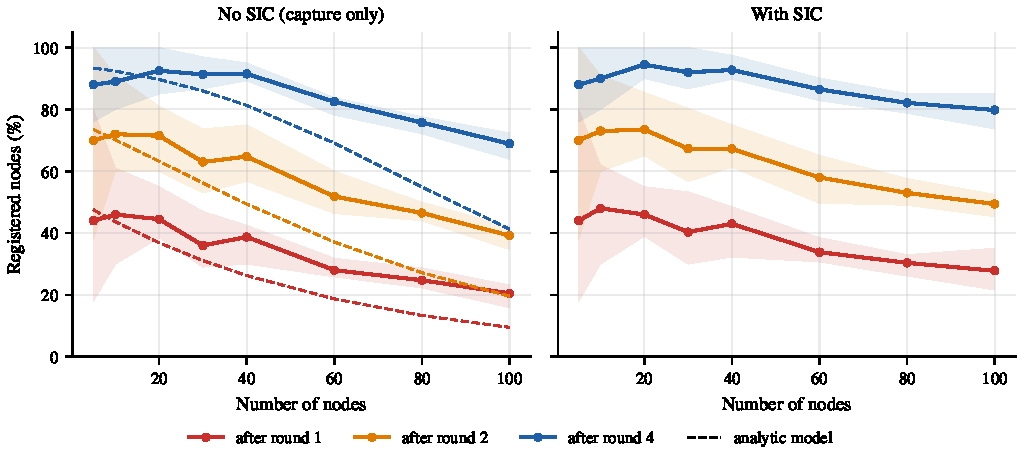
\includegraphics[width=\linewidth]{fig_registration}
\caption{Percentage of nodes registered after one, two and four discovery rounds against node count; mean over 10 runs with a $10$--$90\%$ band; left without SIC, right with SIC. Dashed: the mean-field model of Eq.~\eqref{eq:meanfield} with $p_a=\tfrac12$, $S=10$, $K=3$. This is \emph{our} re-creation of the paper's experiment (the paper's frame length and number of rounds are unknown), so only the qualitative trend is comparable.}
\label{fig:registration}
\end{figure}

Three observations from Figure~\ref{fig:registration}.
\begin{enumerate}
 \item \textbf{The trend reproduces the paper's.} Registration falls monotonically with density: after four rounds $\approx88\%$ at $5$ nodes, but only $69\%$ (no SIC) or $80\%$ (SIC) at $100$ nodes. More rounds recover more nodes (the paper does not say how many rounds it used).
 \item \textbf{At 5 nodes only $\approx44\%$ register in round one---not $\approx100\%$.} With five nodes collisions are rare, so something else limits participation. That something is $p_a\approx\tfrac12$: the base station advertises the slots of the \emph{current and the next} frame, and a node that picks one in the next frame is re-drawn by the next command and effectively sits the round out (Chapter~\ref{ch:bsengine}). The per-round gain then follows $1-0.5^k$: $50\%,75\%,87.5\%$; we measured $44\%,70\%,82\%,88\%$.
 \item \textbf{The model is a lower bound that tracks the shape.} It agrees at low density ($47.5\%$ against $44\%$ at $n=5$, round~1), then falls below the simulation at high density ($9.5\%$ against $21$--$28\%$ at $n=100$, round~1) because it ignores capture, SIC and the $5$~ms rule.
\end{enumerate}

\begin{reality}[Why even five nodes may not all register in one frame]
Observation~2 is not a radio effect at all. It is a consequence of the engine's two-frame RX look-ahead combined with a uniform random choice over the advertised slots. A protocol designer who tunes $S$ by Eq.~\eqref{eq:psucc} will find that the effective number of slots seen by a node is \emph{the advertised list}, i.e.\ twice the frame size, of which only half lie in the current frame. We discuss this in detail in Chapter~\ref{ch:bsengine}.
\end{reality}

\section{Design principles for energy-aware protocols}
\label{sec:principles2}

Putting the pieces together suggests a short checklist, each item testable in Amber.
\begin{enumerate}
 \item \textbf{Don't waste transmissions.} Prefer polls (no collisions) once nodes are known; during discovery, use frames somewhat larger than the expected number of contenders (Section~\ref{sec:energytwist}).
 \item \textbf{Exploit frequency orthogonality.} Assign shifts to spread nodes; collisions then occur only within a group.
 \item \textbf{Use the capture/SIC gain.} Near--far diversity is free; do not assume a collision is a loss.
 \item \textbf{Respect duty cycles.} A node is reachable only for a fraction $D=P_{\mathrm{in}}/P_{\mathrm{act}}$ of the time (Eq.~\eqref{eq:duty}); schedule redundancy accordingly.
 \item \textbf{Adapt.} Estimate the active population from observed outcomes (the custom demo's loop) and resize frames.
\end{enumerate}

\section{Chapter summary}
\begin{itemize}
 \item Ambient IoT protocols are reader-driven; Amber's default one has three commands (\code{send_id}, \code{ack}, \code{send_data}) and three node states (idle, wait\_ack, registered).
 \item Broadcast polling is cheap in commands but collides; unicast polling never collides but costs $N$ commands. The shipped unicast demo answers only $\approx9\%$ of polls: it is energy-limited.
 \item The base station cannot observe node energy states; silent nodes are ambiguous.
 \item A mean-field FSA model gives a lower bound on registration; our re-creation of the paper's experiment reproduces its downward trend.
 \item Engine behaviour (two-frame look-ahead) halves per-round participation: $\approx44\%$ registered after one round even at five nodes.
\end{itemize}

\begin{codemap}
\small
\begin{tabularx}{\linewidth}{@{}>{\ttfamily}p{5.2cm}X@{}}
\toprule
\normalfont\bfseries Concept & \normalfont\bfseries Code\\
\midrule
Command handling & \codew{BackscatterModule.handle_command}\\
Node protocol states & \codew{BackscatterModule.state}: \code{idle}, \code{wait_ack}, \code{registered}\\
ACK delivery & \codew{BSBehavior._send_pending_acks}\\
Pending / registered lists & \codew{nodes_pending_ack}, \codew{nodes_registered}\\
Broadcast vs unicast & \code{target} field: $-1$, int, or list\\
\bottomrule
\end{tabularx}
\end{codemap}

\section*{Exercises}
\begin{exercise}
Using Eq.~\eqref{eq:meanfield} with $p_a=1$, $S=10$, $K=3$ and $n_1=50$, compute the expected registered fraction after one round. Repeat with $p_a=\tfrac12$. By how many rounds does the latter lag?
\end{exercise}
\begin{exercise}
A unicast round for $N$ nodes takes $N(T_{\mathrm{cmd}}+T_{\mathrm{slot}})$. For $T_{\mathrm{cmd}}=5$~ms, $T_{\mathrm{slot}}=10$~ms and $N=100$, how long is a round? If each node can transmit at most once every $2$~s on average, what fraction of polls will be answered?
\end{exercise}
\begin{exercise}
Argue why unicast polling may nonetheless be preferable to broadcast even though it needs $N$ commands. Consider energy per delivered packet (Section~\ref{sec:energytwist}).
\end{exercise}
\begin{exercise}
List three observable quantities from which a base station could infer that a silent node is asleep rather than out of range, and say what each would cost the node.
\end{exercise}
